% Options for packages loaded elsewhere
\PassOptionsToPackage{unicode}{hyperref}
\PassOptionsToPackage{hyphens}{url}
%
\documentclass[
]{article}
\usepackage{amsmath,amssymb}
\usepackage{iftex}
\ifPDFTeX
  \usepackage[T1]{fontenc}
  \usepackage[utf8]{inputenc}
  \usepackage{textcomp} % provide euro and other symbols
\else % if luatex or xetex
  \usepackage{unicode-math} % this also loads fontspec
  \defaultfontfeatures{Scale=MatchLowercase}
  \defaultfontfeatures[\rmfamily]{Ligatures=TeX,Scale=1}
\fi
\usepackage{lmodern}
\ifPDFTeX\else
  % xetex/luatex font selection
\fi
% Use upquote if available, for straight quotes in verbatim environments
\IfFileExists{upquote.sty}{\usepackage{upquote}}{}
\IfFileExists{microtype.sty}{% use microtype if available
  \usepackage[]{microtype}
  \UseMicrotypeSet[protrusion]{basicmath} % disable protrusion for tt fonts
}{}
\makeatletter
\@ifundefined{KOMAClassName}{% if non-KOMA class
  \IfFileExists{parskip.sty}{%
    \usepackage{parskip}
  }{% else
    \setlength{\parindent}{0pt}
    \setlength{\parskip}{6pt plus 2pt minus 1pt}}
}{% if KOMA class
  \KOMAoptions{parskip=half}}
\makeatother
\usepackage{xcolor}
\usepackage[margin=1in]{geometry}
\usepackage{color}
\usepackage{fancyvrb}
\newcommand{\VerbBar}{|}
\newcommand{\VERB}{\Verb[commandchars=\\\{\}]}
\DefineVerbatimEnvironment{Highlighting}{Verbatim}{commandchars=\\\{\}}
% Add ',fontsize=\small' for more characters per line
\usepackage{framed}
\definecolor{shadecolor}{RGB}{248,248,248}
\newenvironment{Shaded}{\begin{snugshade}}{\end{snugshade}}
\newcommand{\AlertTok}[1]{\textcolor[rgb]{0.94,0.16,0.16}{#1}}
\newcommand{\AnnotationTok}[1]{\textcolor[rgb]{0.56,0.35,0.01}{\textbf{\textit{#1}}}}
\newcommand{\AttributeTok}[1]{\textcolor[rgb]{0.13,0.29,0.53}{#1}}
\newcommand{\BaseNTok}[1]{\textcolor[rgb]{0.00,0.00,0.81}{#1}}
\newcommand{\BuiltInTok}[1]{#1}
\newcommand{\CharTok}[1]{\textcolor[rgb]{0.31,0.60,0.02}{#1}}
\newcommand{\CommentTok}[1]{\textcolor[rgb]{0.56,0.35,0.01}{\textit{#1}}}
\newcommand{\CommentVarTok}[1]{\textcolor[rgb]{0.56,0.35,0.01}{\textbf{\textit{#1}}}}
\newcommand{\ConstantTok}[1]{\textcolor[rgb]{0.56,0.35,0.01}{#1}}
\newcommand{\ControlFlowTok}[1]{\textcolor[rgb]{0.13,0.29,0.53}{\textbf{#1}}}
\newcommand{\DataTypeTok}[1]{\textcolor[rgb]{0.13,0.29,0.53}{#1}}
\newcommand{\DecValTok}[1]{\textcolor[rgb]{0.00,0.00,0.81}{#1}}
\newcommand{\DocumentationTok}[1]{\textcolor[rgb]{0.56,0.35,0.01}{\textbf{\textit{#1}}}}
\newcommand{\ErrorTok}[1]{\textcolor[rgb]{0.64,0.00,0.00}{\textbf{#1}}}
\newcommand{\ExtensionTok}[1]{#1}
\newcommand{\FloatTok}[1]{\textcolor[rgb]{0.00,0.00,0.81}{#1}}
\newcommand{\FunctionTok}[1]{\textcolor[rgb]{0.13,0.29,0.53}{\textbf{#1}}}
\newcommand{\ImportTok}[1]{#1}
\newcommand{\InformationTok}[1]{\textcolor[rgb]{0.56,0.35,0.01}{\textbf{\textit{#1}}}}
\newcommand{\KeywordTok}[1]{\textcolor[rgb]{0.13,0.29,0.53}{\textbf{#1}}}
\newcommand{\NormalTok}[1]{#1}
\newcommand{\OperatorTok}[1]{\textcolor[rgb]{0.81,0.36,0.00}{\textbf{#1}}}
\newcommand{\OtherTok}[1]{\textcolor[rgb]{0.56,0.35,0.01}{#1}}
\newcommand{\PreprocessorTok}[1]{\textcolor[rgb]{0.56,0.35,0.01}{\textit{#1}}}
\newcommand{\RegionMarkerTok}[1]{#1}
\newcommand{\SpecialCharTok}[1]{\textcolor[rgb]{0.81,0.36,0.00}{\textbf{#1}}}
\newcommand{\SpecialStringTok}[1]{\textcolor[rgb]{0.31,0.60,0.02}{#1}}
\newcommand{\StringTok}[1]{\textcolor[rgb]{0.31,0.60,0.02}{#1}}
\newcommand{\VariableTok}[1]{\textcolor[rgb]{0.00,0.00,0.00}{#1}}
\newcommand{\VerbatimStringTok}[1]{\textcolor[rgb]{0.31,0.60,0.02}{#1}}
\newcommand{\WarningTok}[1]{\textcolor[rgb]{0.56,0.35,0.01}{\textbf{\textit{#1}}}}
\usepackage{graphicx}
\makeatletter
\def\maxwidth{\ifdim\Gin@nat@width>\linewidth\linewidth\else\Gin@nat@width\fi}
\def\maxheight{\ifdim\Gin@nat@height>\textheight\textheight\else\Gin@nat@height\fi}
\makeatother
% Scale images if necessary, so that they will not overflow the page
% margins by default, and it is still possible to overwrite the defaults
% using explicit options in \includegraphics[width, height, ...]{}
\setkeys{Gin}{width=\maxwidth,height=\maxheight,keepaspectratio}
% Set default figure placement to htbp
\makeatletter
\def\fps@figure{htbp}
\makeatother
\setlength{\emergencystretch}{3em} % prevent overfull lines
\providecommand{\tightlist}{%
  \setlength{\itemsep}{0pt}\setlength{\parskip}{0pt}}
\setcounter{secnumdepth}{-\maxdimen} % remove section numbering
\ifLuaTeX
  \usepackage{selnolig}  % disable illegal ligatures
\fi
\IfFileExists{bookmark.sty}{\usepackage{bookmark}}{\usepackage{hyperref}}
\IfFileExists{xurl.sty}{\usepackage{xurl}}{} % add URL line breaks if available
\urlstyle{same}
\hypersetup{
  pdftitle={Assignment 6: VAR Models},
  pdfauthor={Rachel Montgomery},
  hidelinks,
  pdfcreator={LaTeX via pandoc}}

\title{Assignment 6: VAR Models}
\author{Rachel Montgomery}
\date{2023-10-08}

\begin{document}
\maketitle

\hypertarget{assignment-6-unraveling-multivariate-time-series-with-vector-autoregression}{%
\subsection{Assignment 6: Unraveling Multivariate Time Series with
Vector
Autoregression}\label{assignment-6-unraveling-multivariate-time-series-with-vector-autoregression}}

Time series forecasting is a crucial part of many sectors, from
predicting stock prices to anticipating energy demand. In this
assignment, we'll explore the power of vector autoregression (VAR)
models and learn how to forecast time series data effectively using R.

\hypertarget{section-1-data-exploration}{%
\subsubsection{Section 1: Data
Exploration}\label{section-1-data-exploration}}

Our analysis begins by setting up our data and understanding its key
components.

\hypertarget{loading-and-formatting-data}{%
\paragraph{Loading and Formatting
Data}\label{loading-and-formatting-data}}

We start by loading the ``nashville\_housing'' and
``housing\_validation'' dataset and converting them into a tsibble
format. Additionally, we create a pandemic dummy variable to account for
the impact of the COVID-19 pandemic.

\begin{Shaded}
\begin{Highlighting}[]
\CommentTok{\#load in nashville housing }
\NormalTok{nashville\_housing }\OtherTok{\textless{}{-}} \FunctionTok{read.csv}\NormalTok{(}\StringTok{"nashville\_housing.csv"}\NormalTok{)}

\CommentTok{\# convert date }
\NormalTok{nashville\_housing}\SpecialCharTok{$}\NormalTok{date }\OtherTok{\textless{}{-}} \FunctionTok{yearmonth}\NormalTok{(nashville\_housing}\SpecialCharTok{$}\NormalTok{date)}

\CommentTok{\# Convert to \textasciigrave{}tsibble\textasciigrave{}}
\NormalTok{housing\_ts }\OtherTok{\textless{}{-}}\NormalTok{ nashville\_housing }\SpecialCharTok{\%\textgreater{}\%}
  \FunctionTok{as\_tsibble}\NormalTok{(}\AttributeTok{index =}\NormalTok{ date)}

\CommentTok{\# Set pandemic}
\NormalTok{housing\_ts}\SpecialCharTok{$}\NormalTok{pandemic }\OtherTok{\textless{}{-}} \FunctionTok{rep}\NormalTok{(}\DecValTok{0}\NormalTok{, }\FunctionTok{nrow}\NormalTok{(housing\_ts))}
\NormalTok{housing\_ts}\SpecialCharTok{$}\NormalTok{pandemic[}
  \FunctionTok{which}\NormalTok{(}
    \FunctionTok{as.character}\NormalTok{(housing\_ts}\SpecialCharTok{$}\NormalTok{date) }\SpecialCharTok{==} \StringTok{"2020 May"}
\NormalTok{  )}\SpecialCharTok{:}\FunctionTok{which}\NormalTok{(}
    \FunctionTok{as.character}\NormalTok{(housing\_ts}\SpecialCharTok{$}\NormalTok{date) }\SpecialCharTok{==} \StringTok{"2021 Jun"}
\NormalTok{  )}
\NormalTok{] }\OtherTok{\textless{}{-}} \DecValTok{1}
\end{Highlighting}
\end{Shaded}

For validation purposes, we'll also prepare a validation dataset.

\hypertarget{section-2-building-a-var-model-with-fpp3}{%
\subsubsection{Section 2: Building a VAR Model with
\{fpp3\}}\label{section-2-building-a-var-model-with-fpp3}}

The real fun begins as we attempt to model our multivariate time series
data using VAR.

\hypertarget{fitting-a-var-model}{%
\paragraph{Fitting a VAR Model}\label{fitting-a-var-model}}

Let's fit a VAR model using the \{fpp3\} package to the housing data and
examine how well it captures the data's dynamics.

\begin{Shaded}
\begin{Highlighting}[]
\CommentTok{\# Fit VAR model}

\NormalTok{fit\_var }\OtherTok{\textless{}{-}}\NormalTok{ housing\_ts }\SpecialCharTok{\%\textgreater{}\%}
  \FunctionTok{model}\NormalTok{(}
    \AttributeTok{var\_model =} \FunctionTok{VAR}\NormalTok{(}
      \FunctionTok{vars}\NormalTok{(housing, unemployment, median\_days, price\_increased, price\_decreased, pending\_listing, median\_price) }\SpecialCharTok{\textasciitilde{}}
        \FunctionTok{xreg}\NormalTok{(pandemic)}
\NormalTok{      )}
\NormalTok{    )}
\end{Highlighting}
\end{Shaded}

\hypertarget{reporting-model-fit}{%
\paragraph{Reporting Model Fit}\label{reporting-model-fit}}

Understanding how well our model fits the data is essential. Let's
inspect the fit.

\begin{Shaded}
\begin{Highlighting}[]
\CommentTok{\# Report fit}
\CommentTok{\#report(fit\_var) \#\#hiding because output is so long}
\end{Highlighting}
\end{Shaded}

\emph{How many lags were used?}

\hypertarget{autocorrelation-analysis}{%
\paragraph{Autocorrelation Analysis}\label{autocorrelation-analysis}}

\begin{Shaded}
\begin{Highlighting}[]
\CommentTok{\# Autocorrelation of residuals}
\NormalTok{fit\_var }\SpecialCharTok{\%\textgreater{}\%}
  \FunctionTok{augment}\NormalTok{() }\SpecialCharTok{\%\textgreater{}\%}
\FunctionTok{ACF}\NormalTok{(.innov) }\SpecialCharTok{\%\textgreater{}\%}
  \FunctionTok{autoplot}\NormalTok{()}
\end{Highlighting}
\end{Shaded}

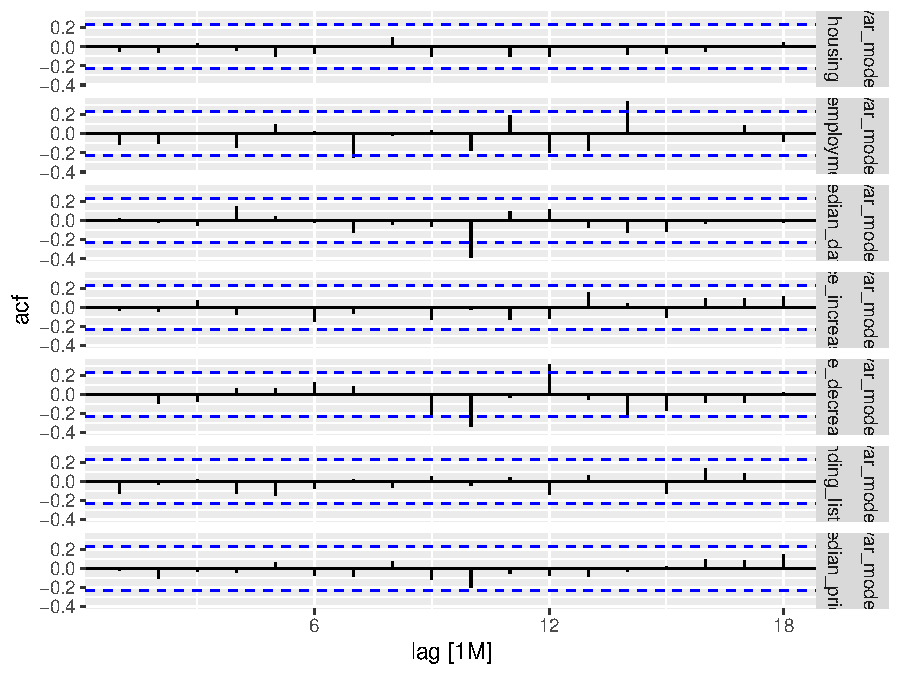
\includegraphics{Montgomery_Rachel_Assignment6_files/figure-latex/unnamed-chunk-5-1.pdf}

To determine if any autocorrelations are significant, we typically look
for bars (lags) that extend beyond the dashed blue lines, which
represent the significance level. If a bar crosses this line, it means
the autocorrelation for that specific lag is statistically significant.

\begin{itemize}
\item
  housing: significant autocorrelation around lag 12.
\item
  price\_increased: significant autocorrelation around lag 12.
\item
  price\_decreased: Significant autocorrelation observed around lag 6
  and 12.
\item
  pending\_listing: Significant autocorrelation around lag 12.
\end{itemize}

\hypertarget{significant-autocorrelations}{%
\paragraph{Significant
Autocorrelations}\label{significant-autocorrelations}}

Identifying significant autocorrelations in the residuals.

\begin{quote}
Report significant autocorrelations. Report all variables and lags that
are significant.
\end{quote}

\hypertarget{section-3-building-a-var-model-with-vars}{%
\subsubsection{Section 3: Building a VAR Model with
\{vars\}}\label{section-3-building-a-var-model-with-vars}}

The heart of this assignment lies in building VAR models to analyze and
forecast our multivariate data.

\hypertarget{fitting-a-var-model-with-vars}{%
\paragraph{Fitting a VAR Model with
\{vars\}}\label{fitting-a-var-model-with-vars}}

We will once again model our housing data, but this time using functions
from the \{vars\} package.

\begin{Shaded}
\begin{Highlighting}[]
\CommentTok{\# VAR model with \{vars\}}

\NormalTok{vars\_var }\OtherTok{\textless{}{-}}\NormalTok{ vars}\SpecialCharTok{::}\FunctionTok{VAR}\NormalTok{(}
  \AttributeTok{y =}\NormalTok{ housing\_ts[,}\FunctionTok{c}\NormalTok{(}
    \StringTok{"housing"}\NormalTok{, }\StringTok{"unemployment"}\NormalTok{, }\StringTok{"median\_days"}\NormalTok{,}
    \StringTok{"price\_decreased"}\NormalTok{, }\StringTok{"pending\_listing"}
\NormalTok{  )],}
  \AttributeTok{exogen =}\NormalTok{ housing\_ts[,}\FunctionTok{c}\NormalTok{(}\StringTok{"pandemic"}\NormalTok{)],}
  \AttributeTok{type =} \StringTok{"none"}\NormalTok{, }\CommentTok{\# same as \{fpp3\}\textquotesingle{}s \textasciigrave{}VAR\textasciigrave{}}
  \AttributeTok{p =} \DecValTok{5} \CommentTok{\# lag}
\NormalTok{)}

\CommentTok{\# Make dummy variable matrix}
\NormalTok{dummat }\OtherTok{\textless{}{-}} \FunctionTok{matrix}\NormalTok{(}
  \FunctionTok{rep}\NormalTok{(}\DecValTok{0}\NormalTok{, }\DecValTok{2} \SpecialCharTok{*} \DecValTok{24}\NormalTok{), }\AttributeTok{nrow =} \DecValTok{24}\NormalTok{,}
  \AttributeTok{dimnames =} \FunctionTok{list}\NormalTok{(}\ConstantTok{NULL}\NormalTok{, }\FunctionTok{c}\NormalTok{(}\StringTok{"outlier"}\NormalTok{, }\StringTok{"pandemic"}\NormalTok{)))}
\end{Highlighting}
\end{Shaded}

\hypertarget{serial-test-on-residual-autocorrelations}{%
\paragraph{Serial Test on Residual
Autocorrelations}\label{serial-test-on-residual-autocorrelations}}

A serial test can give insights into the independence of residuals.

\begin{Shaded}
\begin{Highlighting}[]
\CommentTok{\# Perform serial test}

\CommentTok{\# Fit VAR(2)}
\NormalTok{var\_2 }\OtherTok{\textless{}{-}}\NormalTok{ vars}\SpecialCharTok{::}\FunctionTok{VAR}\NormalTok{(}
\NormalTok{  housing\_ts[,}\SpecialCharTok{{-}}\FunctionTok{c}\NormalTok{(}\DecValTok{1}\NormalTok{, }\DecValTok{9}\NormalTok{)], }\AttributeTok{p =} \DecValTok{2}\NormalTok{, }\AttributeTok{type =} \StringTok{"none"}\NormalTok{, }
  \AttributeTok{exogen =}\NormalTok{ housing\_ts[,}\FunctionTok{c}\NormalTok{(}\DecValTok{9}\NormalTok{)]}
\NormalTok{)}
\FunctionTok{serial.test}\NormalTok{(var\_2, }\AttributeTok{lags.pt =} \DecValTok{4}\NormalTok{, }\AttributeTok{type =} \StringTok{"PT.adjusted"}\NormalTok{)}
\end{Highlighting}
\end{Shaded}

\begin{verbatim}

    Portmanteau Test (adjusted)

data:  Residuals of VAR object var_2
Chi-squared = 151.63, df = 98, p-value = 0.0004178
\end{verbatim}

\begin{Shaded}
\begin{Highlighting}[]
\CommentTok{\# Fit VAR(2) with season}
\NormalTok{var\_2\_season }\OtherTok{\textless{}{-}}\NormalTok{ vars}\SpecialCharTok{::}\FunctionTok{VAR}\NormalTok{(}
\NormalTok{  housing\_ts[,}\SpecialCharTok{{-}}\FunctionTok{c}\NormalTok{(}\DecValTok{1}\NormalTok{, }\DecValTok{9}\NormalTok{)], }\AttributeTok{p =} \DecValTok{2}\NormalTok{, }\AttributeTok{type =} \StringTok{"none"}\NormalTok{, }
  \AttributeTok{exogen =}\NormalTok{ housing\_ts[,}\FunctionTok{c}\NormalTok{(}\DecValTok{9}\NormalTok{)], }\AttributeTok{season =} \DecValTok{12}
\NormalTok{)}
\FunctionTok{serial.test}\NormalTok{(var\_2\_season, }\AttributeTok{lags.pt =} \DecValTok{10}\NormalTok{, }\AttributeTok{type =} \StringTok{"PT.adjusted"}\NormalTok{)}
\end{Highlighting}
\end{Shaded}

\begin{verbatim}

    Portmanteau Test (adjusted)

data:  Residuals of VAR object var_2_season
Chi-squared = 501.17, df = 392, p-value = 0.0001533
\end{verbatim}

\begin{Shaded}
\begin{Highlighting}[]
\DocumentationTok{\#\# Set \textquotesingle{}lags.pt\textquotesingle{} to \textasciigrave{}4\textasciigrave{}}
\DocumentationTok{\#\# Set \textquotesingle{}type\textquotesingle{} to "PT.adjusted"}
\end{Highlighting}
\end{Shaded}

Question: Interpret the p-value from the serial test. What implications
does it have for our model?

\hypertarget{forecasting-with-var}{%
\paragraph{Forecasting with VAR}\label{forecasting-with-var}}

Let's use our VAR model to predict future values.

\begin{Shaded}
\begin{Highlighting}[]
\CommentTok{\# dummy matrix}
\NormalTok{dummat }\OtherTok{\textless{}{-}} \FunctionTok{matrix}\NormalTok{(}
  \FunctionTok{rep}\NormalTok{(}\DecValTok{0}\NormalTok{, }\DecValTok{13}\NormalTok{), }\AttributeTok{nrow =} \DecValTok{13}\NormalTok{,}
  \AttributeTok{dimnames =} \FunctionTok{list}\NormalTok{(}\ConstantTok{NULL}\NormalTok{, }\FunctionTok{c}\NormalTok{(}\StringTok{"pandemic"}\NormalTok{))}
\NormalTok{)}

\CommentTok{\# forecast}
\NormalTok{var\_fc }\OtherTok{\textless{}{-}} \FunctionTok{predict}\NormalTok{(var\_2, }\AttributeTok{n.ahead =} \DecValTok{13}\NormalTok{, }\AttributeTok{dumvar =}\NormalTok{ dummat)}
\end{Highlighting}
\end{Shaded}

\hypertarget{reformatting-forecast}{%
\paragraph{Reformatting forecast}\label{reformatting-forecast}}

Now, let's format and plot our forecast against the validation data.

\hypertarget{plot-the-forecast-against-the-validation-data}{%
\paragraph{Plot the forecast against the validation
data}\label{plot-the-forecast-against-the-validation-data}}

\begin{verbatim}
Plot variable not specified, automatically selected `.vars = .mean`
\end{verbatim}

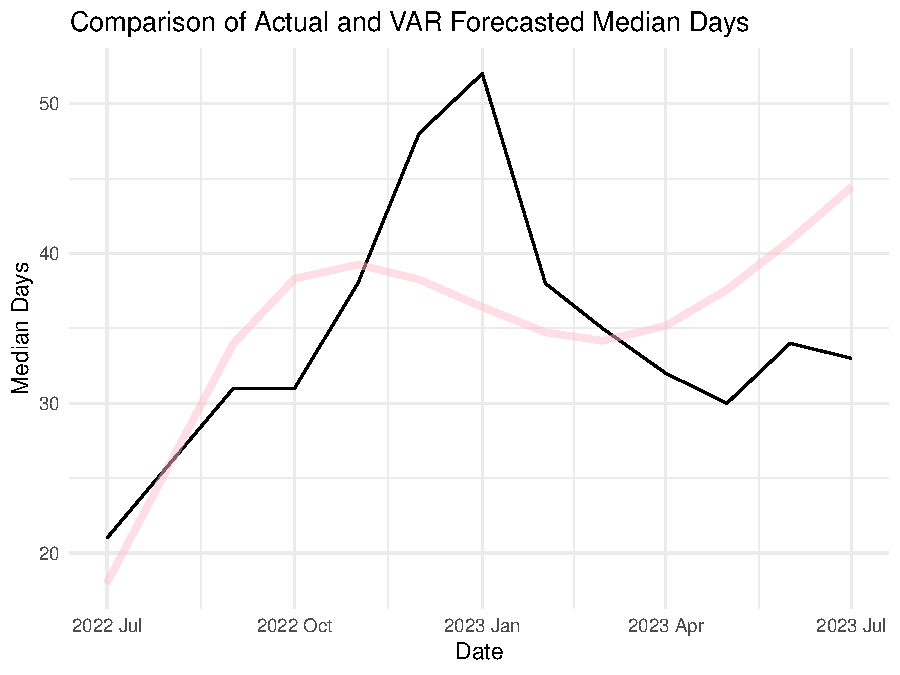
\includegraphics{Montgomery_Rachel_Assignment6_files/figure-latex/unnamed-chunk-10-1.pdf}

\hypertarget{trustworthiness-of-var-forecast}{%
\paragraph{Trustworthiness of VAR
forecast}\label{trustworthiness-of-var-forecast}}

By visually examining the plot, here's an interpretation:

\begin{itemize}
\item
  \textbf{Beginning to late 2022}: The VAR forecast (pink line) closely
  follows the actual \texttt{median\_days} (black line), suggesting that
  the model's forecast was quite accurate for this period.
\item
  \textbf{Late 2022 to early 2023}: The actual values spike
  significantly while the forecasted values only show a mild increase.
  This suggests that the VAR model did not capture this particular
  behavior or event that led to the spike in the actual data.
\item
  \textbf{Mid 2023 onwards}: Post the spike, the actual values decrease
  and then stabilize. The VAR model seems to anticipate this decline but
  not to the same extent as the actual data. The forecast then appears
  to mildly underestimate the actual \texttt{median\_days} values.
\end{itemize}

In conclusion, the VAR forecast appears reasonably accurate at the
beginning of the period. However, it missed the sharp spike and seems to
mildly underestimate the data towards the end.

\hypertarget{section-4-vecm-models}{%
\subsubsection{Section 4: VECM Models}\label{section-4-vecm-models}}

VECM (Vector Error Correction Models) is another method for handling
multivariate time series. Let's explore its capabilities.

\hypertarget{cointegration-analysis}{%
\paragraph{Cointegration Analysis}\label{cointegration-analysis}}

We perform the Johansen Procedure to understand the relationships
between variables and determine the rank of evidence. Cointegration can
help us understand the long-term relationships between our variables.

\begin{Shaded}
\begin{Highlighting}[]
\CommentTok{\# Cointegration}
\NormalTok{co\_test }\OtherTok{\textless{}{-}} \FunctionTok{ca.jo}\NormalTok{(}
  \CommentTok{\# variables}
  \AttributeTok{x =}\NormalTok{ housing\_ts[,}\FunctionTok{c}\NormalTok{(}
    \StringTok{"housing"}\NormalTok{, }\StringTok{"unemployment"}\NormalTok{, }\StringTok{"median\_days"}\NormalTok{,}
    \StringTok{"price\_decreased"}\NormalTok{, }\StringTok{"pending\_listing"}
\NormalTok{  )],  }
  \AttributeTok{type =} \StringTok{"trace"}\NormalTok{, }\CommentTok{\# tends to be more conservative}
  \AttributeTok{K =} \DecValTok{5}\NormalTok{, }\CommentTok{\# lag {-}{-} same as your VAR model}
  \AttributeTok{spec =} \StringTok{"longrun"}\NormalTok{, }\CommentTok{\# generally use "longrun"}
  \AttributeTok{ecdet =} \StringTok{"trend"}\NormalTok{, }\CommentTok{\# trend{-}stationary}
  \CommentTok{\# exogeneous dummy variables}
  \AttributeTok{dumvar =}\NormalTok{ housing\_ts[,}\FunctionTok{c}\NormalTok{(}\StringTok{"pandemic"}\NormalTok{)]}
\NormalTok{)}
\end{Highlighting}
\end{Shaded}

\hypertarget{discussion-of-cointegration-analysis}{%
\paragraph{Discussion of Cointegration
Analysis}\label{discussion-of-cointegration-analysis}}

Now, let's discuss the results.

\begin{Shaded}
\begin{Highlighting}[]
\NormalTok{co\_summ }\OtherTok{\textless{}{-}} \FunctionTok{summary}\NormalTok{(co\_test)}
\end{Highlighting}
\end{Shaded}

\emph{To determine the rank for which we have evidence of
cointegration:}

\begin{enumerate}
\def\labelenumi{\arabic{enumi}.}
\item
  To determine the rank for which we have evidence of cointegration:
\item
  Start from the bottom (r = 0) and move upwards. Compare the test
  statistic to the critical values.
\end{enumerate}

\emph{The results are:}

\begin{itemize}
\item
  r \(≤\) 4: The test statistic is 0.06, which is less than the critical
  values at all significance levels (10.49, 12.25, 16.26). Therefore, we
  do not reject the hypothesis that r ≤ 4.
\item
  r \(≤\) 3: The test statistic is 6.59, which is less than the critical
  values at all significance levels (22.76, 25.32, 30.45). So, we do not
  reject the hypothesis that r ≤ 3.
\item
  r \(≤\) 2: The test statistic is 24.16, which is less than the
  critical values at all significance levels (39.06, 42.44, 48.45). So,
  we do not reject the hypothesis that r ≤ 2.
\item
  r \(≤\) 1: The test statistic is 51.79, which is less than the
  critical values at the 1\% significance level (70.05) but is below the
  critical values at the 5\% and 10\% significance levels. So, we reject
  the hypothesis that r ≤ 1 at the 10\% and 5\% significance levels.
\item
  r = 0: The test statistic is 94.60, which is greater than the critical
  values at all significance levels (83.20, 87.31, 96.58). We can reject
  the hypothesis that r = 0 at the 10\% and 5\% significance levels but
  not at the 1\% significance level.
\end{itemize}

\emph{Conclusion:} We have evidence for a rank of 1 at the 5\%
significance level. The test statistic for this rank is 51.79. The
critical value for this rank at the 5\% significance level is 62.99.

\hypertarget{converting-to-var-and-additional-forecasting}{%
\paragraph{Converting to VAR and Additional
Forecasting}\label{converting-to-var-and-additional-forecasting}}

We convert our VECM to VAR and conduct further forecasting. We compare
the VECM and VAR forecasts to make informed decisions.

\begin{Shaded}
\begin{Highlighting}[]
\CommentTok{\# Convert VECM to VAR}
\NormalTok{vecm }\OtherTok{\textless{}{-}}\NormalTok{ vars}\SpecialCharTok{::}\FunctionTok{vec2var}\NormalTok{(co\_test, }\AttributeTok{r =} \DecValTok{2}\NormalTok{)}

\CommentTok{\# Make dummy variable matrix}
\NormalTok{dummy\_var\_matrix }\OtherTok{\textless{}{-}} \FunctionTok{matrix}\NormalTok{(}
  \FunctionTok{rep}\NormalTok{(}\DecValTok{0}\NormalTok{, }\DecValTok{1} \SpecialCharTok{*} \DecValTok{13}\NormalTok{), }\AttributeTok{nrow =} \DecValTok{13}\NormalTok{,}
  \AttributeTok{dimnames =} \FunctionTok{list}\NormalTok{(}\ConstantTok{NULL}\NormalTok{, }\FunctionTok{c}\NormalTok{(}\StringTok{"pandemic"}\NormalTok{)))}

\CommentTok{\# Forecast}
\NormalTok{vecm\_forecast }\OtherTok{\textless{}{-}} \FunctionTok{predict}\NormalTok{(vecm, }\AttributeTok{n.ahead =} \DecValTok{13}\NormalTok{, }\AttributeTok{dumvar =}\NormalTok{ dummy\_var\_matrix)}
\end{Highlighting}
\end{Shaded}

\hypertarget{reformatting-forecast-1}{%
\paragraph{Reformatting forecast}\label{reformatting-forecast-1}}

Use housing\_validation's date variable, we'll format the median\_days
forecast to \{fpp3\} specifications.

\begin{Shaded}
\begin{Highlighting}[]
\CommentTok{\# Get forecast values}
\NormalTok{fc\_median\_days }\OtherTok{\textless{}{-}}\NormalTok{ vecm\_forecast}\SpecialCharTok{$}\NormalTok{fcst}\SpecialCharTok{$}\NormalTok{median\_days}

\CommentTok{\# Set up forecast as \{fpp3\} does}
\NormalTok{vecm\_fc }\OtherTok{\textless{}{-}} \FunctionTok{data.frame}\NormalTok{(}
  \AttributeTok{.model =} \StringTok{"VECM"}\NormalTok{,}
  \AttributeTok{date =}\NormalTok{ validation\_ts}\SpecialCharTok{$}\NormalTok{date,}
  \AttributeTok{median\_days =}\NormalTok{ distributional}\SpecialCharTok{::}\FunctionTok{dist\_normal}\NormalTok{(}
    \AttributeTok{mean =}\NormalTok{ fc\_median\_days[,}\StringTok{"fcst"}\NormalTok{],}
    \AttributeTok{sd =}\NormalTok{ fc\_median\_days[,}\StringTok{"CI"}\NormalTok{]}
\NormalTok{  ),}
  \AttributeTok{.mean =}\NormalTok{ fc\_median\_days[,}\StringTok{"fcst"}\NormalTok{]}
\NormalTok{) }\SpecialCharTok{\%\textgreater{}\%} \FunctionTok{as\_tsibble}\NormalTok{(}\AttributeTok{index =}\NormalTok{ date)}

\CommentTok{\# Add "housing" to dimnames}
\FunctionTok{dimnames}\NormalTok{(vecm\_fc}\SpecialCharTok{$}\NormalTok{median\_days) }\OtherTok{\textless{}{-}} \StringTok{"median\_days"}
\end{Highlighting}
\end{Shaded}

\hypertarget{plot-the-vecm-forecast-against-the-validation-data-and-var-forecast}{%
\paragraph{\texorpdfstring{Plot the VECM forecast against the validation
data and \texttt{VAR}
forecast}{Plot the VECM forecast against the validation data and VAR forecast}}\label{plot-the-vecm-forecast-against-the-validation-data-and-var-forecast}}

With our VAR models in place, it's time to evaluate their performance
and use them for forecasting.

\begin{Shaded}
\begin{Highlighting}[]
\NormalTok{validation\_ts }\SpecialCharTok{\%\textgreater{}\%}
  \FunctionTok{autoplot}\NormalTok{(median\_days) }\SpecialCharTok{+}
  \FunctionTok{autolayer}\NormalTok{(var\_fc, }\AttributeTok{alpha =} \FloatTok{0.5}\NormalTok{, }\AttributeTok{size =} \FloatTok{1.5}\NormalTok{, }\AttributeTok{color =} \StringTok{"pink"}\NormalTok{) }\SpecialCharTok{+} 
  \FunctionTok{autolayer}\NormalTok{(vecm\_fc, }\AttributeTok{alpha =} \FloatTok{0.5}\NormalTok{, }\AttributeTok{size =} \FloatTok{1.5}\NormalTok{, }\AttributeTok{color =} \StringTok{"purple"}\NormalTok{) }\SpecialCharTok{+} 
  \FunctionTok{labs}\NormalTok{(}\AttributeTok{title =} \StringTok{"Comparison of Actual, VAR and VECM Forecasted Median Days"}\NormalTok{,}
       \AttributeTok{x =} \StringTok{"Date"}\NormalTok{,}
       \AttributeTok{y =} \StringTok{"Median Days"}\NormalTok{) }\SpecialCharTok{+}
  \FunctionTok{theme\_minimal}\NormalTok{()}
\end{Highlighting}
\end{Shaded}

\begin{verbatim}
## Plot variable not specified, automatically selected `.vars = .mean`
## Plot variable not specified, automatically selected `.vars = .mean`
\end{verbatim}

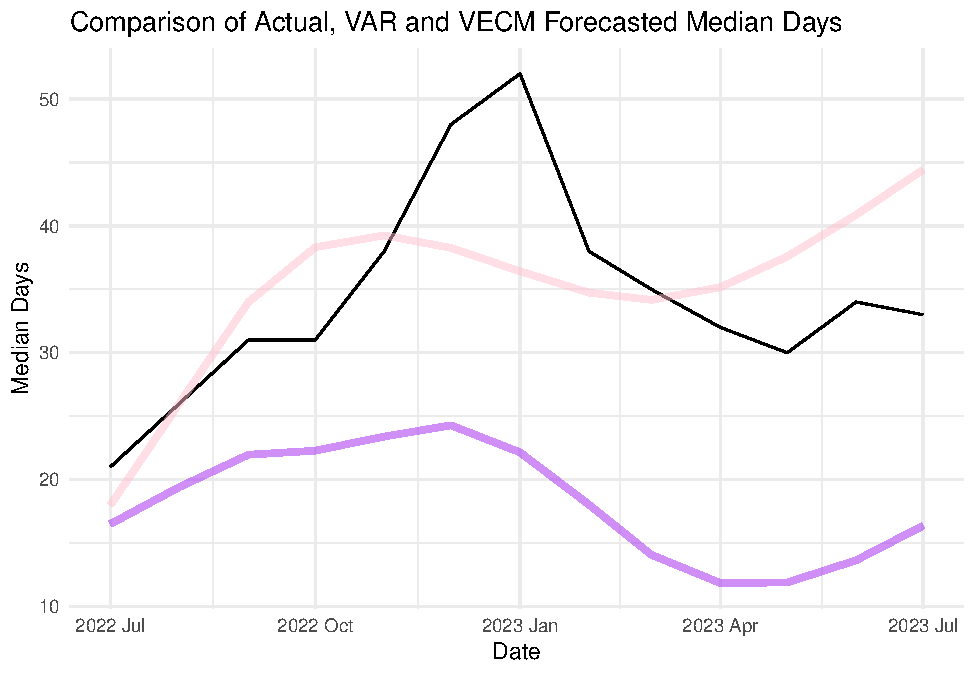
\includegraphics{Montgomery_Rachel_Assignment6_files/figure-latex/unnamed-chunk-15-1.pdf}

\hypertarget{section-4-model-comparison-and-conclusion}{%
\subsubsection{Section 4: Model Comparison and
Conclusion}\label{section-4-model-comparison-and-conclusion}}

\hypertarget{comparing-forecasts}{%
\paragraph{Comparing Forecasts}\label{comparing-forecasts}}

Based on the plotted forecasts, I prefer the VECM model.

\begin{itemize}
\item
  The VECM forecast (in purple) seems to capture the trend of the actual
  data more closely than the VAR forecast (in pink), especially around
  the peak observed around January 2023.
\item
  The VECM also appears to be less volatile than the VAR model.
\end{itemize}

\hypertarget{conclusion}{%
\subsubsection{Conclusion}\label{conclusion}}

\end{document}
